\documentclass[11pt, letterpaper]{article}
\usepackage[utf8]{inputenc}
\usepackage[margin=1in]{geometry}
\usepackage{amsmath}
\usepackage{amssymb}
\usepackage{tikz}
\usepackage{pgfplots}
\pgfplotsset{compat=1.18}
\usepackage{float}
\usepackage{enumitem}
\usepackage{titlesec}

% Title Formatting
\titleformat{\section}{\large\bfseries}{\thesection}{1em}{}
\titleformat{\subsection}{\normalsize\bfseries}{\thesubsection}{1em}{}

% Meta Data
\title{\textbf{ECON 315: International Economics \\ Problem Set \#1}}
\author{Sean Balbale \\ Trinity College (Class of '27)}
\date{February 5, 2026}

\begin{document}

\maketitle

\section*{Problem 1}

\textbf{Given Data:}
\begin{center}
  \begin{tabular}{|l|c|c|}
    \hline
    & \textbf{U.S.} & \textbf{Chile} \\
    \hline
    Wheat (bushels/labor hr) & 6 & 1 \\
    \hline
    Cloth (yards/labor hr) & 4 & 3 \\
    \hline
  \end{tabular}
\end{center}

\subsection*{(a) Absolute Advantage}
\textbf{Restatement:} Does the U.S. or Chile have an absolute advantage in wheat or cloth?

\noindent \textbf{Solution:}
\begin{itemize}
  \item \textbf{Wheat:} The U.S. has an absolute advantage. One hour of labor produces 6 bushels in the U.S. versus only 1 bushel in Chile.
  \item \textbf{Cloth:} The U.S. has an absolute advantage. One hour of labor produces 4 yards in the U.S. versus 3 yards in Chile.
\end{itemize}

\subsection*{(b) Comparative Advantage}
\textbf{Restatement:} In which commodity does the U.S. and Chile have a relative advantage and why?

\noindent \textbf{Solution:}
\begin{itemize}
  \item \textbf{United States (Wheat):} The U.S. has a comparative advantage in Wheat.
    \begin{itemize}
      \item \textit{Reasoning:} The opportunity cost of 1 bushel of Wheat in the U.S. is $4/6 = 0.67$ yards of Cloth. In Chile, it is $3/1 = 3$ yards of Cloth. Since the U.S. has a lower opportunity cost ($0.67 < 3$), it should specialize in Wheat.
    \end{itemize}
  \item \textbf{Chile (Cloth):} Chile has a comparative advantage in Cloth.
    \begin{itemize}
      \item \textit{Reasoning:} The opportunity cost of 1 yard of Cloth in Chile is $1/3 = 0.33$ bushels of Wheat. In the U.S., it is $6/4 = 1.5$ bushels of Wheat. Since Chile has a lower opportunity cost ($0.33 < 1.5$), it should specialize in Cloth.
    \end{itemize}
\end{itemize}

\subsection*{(c) Gains from Trade}
\textbf{Restatement:} Calculate the gains from trade for the U.S. and Chile under three terms of trade: $6W=6C$, $6W=18C$, and $6W=4C$.

\noindent \textbf{Solution:}

\noindent \textbf{1. Scenario $6W = 6C$ ($1W = 1C$):}
\begin{itemize}
  \item \textbf{U.S. Gains:} Exports 6W. In autarky, 6W is worth 4C. With trade, receives 6C. \\ \textbf{Gain = 2C} ($6 - 4$).
  \item \textbf{Chile Gains:} Imports 6W. In autarky, 6W costs 18C ($6 \times 3$). With trade, pays 6C. \\ \textbf{Gain = 12C} ($18 - 6$).
\end{itemize}

\noindent \textbf{2. Scenario $6W = 18C$ ($1W = 3C$):}
\begin{itemize}
  \item \textbf{U.S. Gains:} Exports 6W. Receives 18C. Autarky value was 4C. \\ \textbf{Gain = 14C} ($18 - 4$).
  \item \textbf{Chile Gains:} Imports 6W. Pays 18C. Autarky cost was 18C. \\ \textbf{Gain = 0}. (Terms match Chile's internal opportunity cost).
\end{itemize}

\noindent \textbf{3. Scenario $6W = 4C$ ($1W = 0.67C$):}
\begin{itemize}
  \item \textbf{U.S. Gains:} Exports 6W. Receives 4C. Autarky value was 4C. \\ \textbf{Gain = 0}. (Terms match U.S. internal opportunity cost).
  \item \textbf{Chile Gains:} Imports 6W. Pays 4C. Autarky cost was 18C. \\ \textbf{Gain = 14C} ($18 - 4$).
\end{itemize}

\subsection*{(d) Opportunity Costs \& Trading Range}
\textbf{Restatement:} Now express the table in terms of opportunity costs for
both countries, viz., the relative price of wheat in terms of cloth and the
relative price of cloth in terms of wheat. Indicate the permissible trading
range for $P_w/P_c$ and $P_c/P_w$.

\noindent \textbf{Solution:}
\begin{center}
  \begin{tabular}{|l|c|c|}
    \hline
    & \textbf{U.S. Opp. Cost} & \textbf{Chile Opp. Cost} \\
    \hline
    1 Wheat & $2/3$ Cloth (0.67C) & 3 Cloth \\
    \hline
    1 Cloth & $3/2$ Wheat (1.5W) & $1/3$ Wheat (0.33W) \\
    \hline
  \end{tabular}
\end{center}

\noindent \textbf{Permissible Trading Range:}
\begin{itemize}
  \item For Wheat ($P_W/P_C$): $0.67C < P_W < 3C$
  \item For Cloth ($P_C/P_W$): $0.33W < P_C < 1.5W$
\end{itemize}

\subsection*{(e) Labor Content \& Prices}
\textbf{Restatement:} Using the information in the table, assume that labor is the only factor of production and is homogenous (i.e., of uniform quality). What is the cost in terms of labor content of producing one bushel of wheat and one yard of cloth in the U.S. and Chile? What is the dollar price of wheat and cloth in the U.S. if the wage rate is \$6? What is the peso price of wheat and cloth in Chile if the wage rate is Ps 10?

\noindent \textbf{Solution:}
\begin{itemize}
  \item \textbf{Labor Content:}
    \begin{itemize}
      \item U.S.: 1 Wheat = $1/6$ hr; 1 Cloth = $1/4$ hr.
      \item Chile: 1 Wheat = 1 hr; 1 Cloth = $1/3$ hr.
    \end{itemize}
  \item \textbf{U.S. Dollar Prices:}
    \begin{itemize}
      \item $P_W = \$6 \times (1/6) = \textbf{\$1.00}$
      \item $P_C = \$6 \times (1/4) = \textbf{\$1.50}$
    \end{itemize}
  \item \textbf{Chile Peso Prices:}
    \begin{itemize}
      \item $P_W = 10 \text{ Ps} \times 1 = \textbf{10 Ps}$
      \item $P_C = 10 \text{ Ps} \times (1/3) = \textbf{3.33 Ps}$
    \end{itemize}
\end{itemize}

\subsection*{(f) Production Possibility Curves (PPC)}
\textbf{Restatement:} Suppose now that each country has 100 hrs of labor available to produce either commodity. Construct the production possibilities curves for each country before trade. Put clothing on the horizontal axis and wheat on the vertical axis. What does the slope of each PPC signify before trade takes place? Assume that with the opening of trade the U.S. exchanges 1W for 1C with Chile. Show graphically for the U.S. and Chile the point of production and (possible) consumption with trade, and the gains from trade. Be specific (and careful) in your answer.

\noindent \textbf{Solution:}
\begin{itemize}
  \item \textbf{Slope Significance:} The slope represents the internal \textbf{Opportunity Cost} (MRT) in autarky.
  \item \textbf{U.S. PPC:} Intercepts at 600W ($100 \times 6$) and 400C ($100 \times 4$).
  \item \textbf{Chile PPC:} Intercepts at 100W ($100 \times 1$) and 300C ($100 \times 3$).
\end{itemize}

\begin{figure}[H]
  \centering
  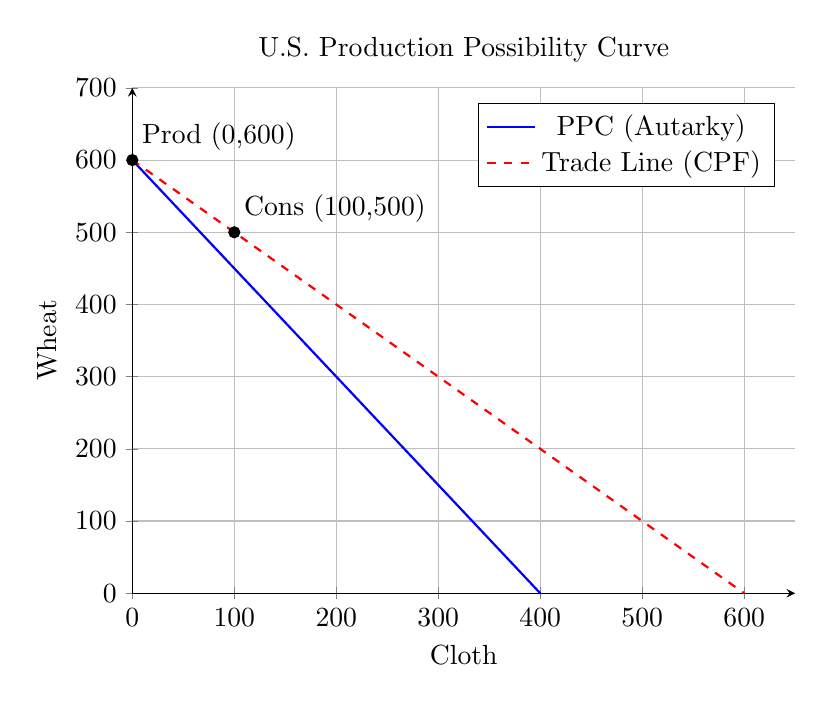
\begin{tikzpicture}
    \begin{axis}[
        title={U.S. Production Possibility Curve},
        xlabel={Cloth},
        ylabel={Wheat},
        xmin=0, xmax=650,
        ymin=0, ymax=700,
        axis lines=left,
        grid=major,
        legend pos=north east,
        width=10cm, height=8cm,
      ]

      % PPC: (0, 600) to (400, 0)
      \addplot[
        color=blue,
        thick,
        domain=0:400,
      ] coordinates {(0,600) (400,0)};
      \addlegendentry{PPC (Autarky)}

      % Trade Line: Slope -1 starting from Production (0, 600)
      % Equation: W = 600 - C
      \addplot[
        color=red,
        dashed,
        thick,
        domain=0:600,
      ] coordinates {(0,600) (600,0)};
      \addlegendentry{Trade Line (CPF)}

      % Production Point A
      \addplot[mark=*] coordinates {(0,600)} node[anchor=south west] {Prod (0,600)};

      % Consumption Point
      \addplot[mark=*] coordinates {(100,500)} node[anchor=south west] {Cons (100,500)};

    \end{axis}
  \end{tikzpicture}
  \caption{U.S. PPC and Consumption with Trade}
\end{figure}

\begin{figure}[H]
  \centering
  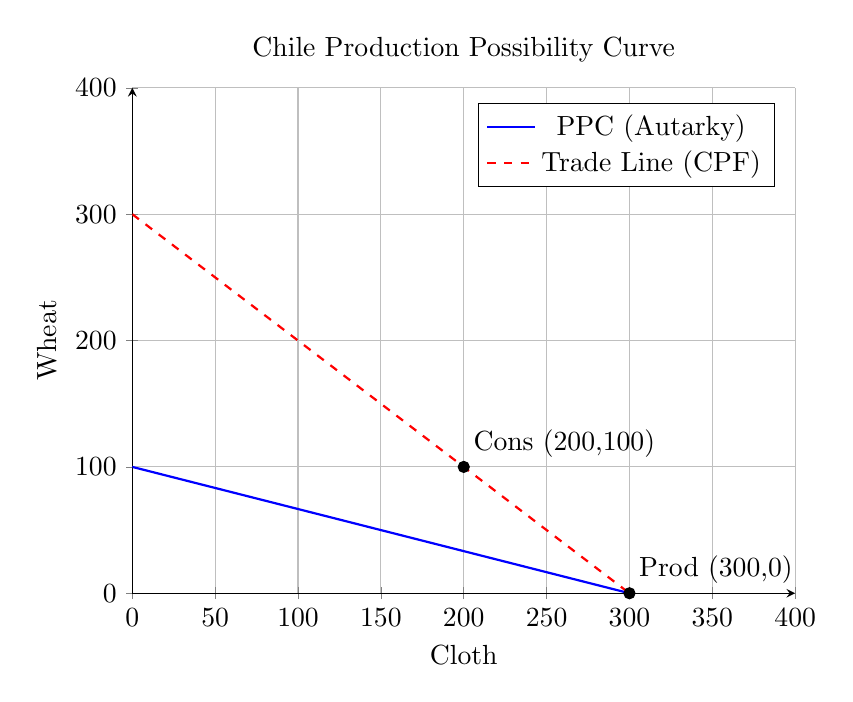
\begin{tikzpicture}
    \begin{axis}[
        title={Chile Production Possibility Curve},
        xlabel={Cloth},
        ylabel={Wheat},
        xmin=0, xmax=400,
        ymin=0, ymax=400,
        axis lines=left,
        grid=major,
        legend pos=north east,
        width=10cm, height=8cm,
      ]

      % PPC: (0, 100) to (300, 0)
      \addplot[
        color=blue,
        thick,
      ] coordinates {(0,100) (300,0)};
      \addlegendentry{PPC (Autarky)}

      % Trade Line: Slope -1 starting from Production (300, 0)
      % Equation: W = 300 - C
      \addplot[
        color=red,
        dashed,
        thick,
      ] coordinates {(0,300) (300,0)};
      \addlegendentry{Trade Line (CPF)}

      % Production Point B'
      \addplot[mark=*] coordinates {(300,0)} node[anchor=south west] {Prod (300,0)};

      % Consumption Point
      \addplot[mark=*] coordinates {(200,100)} node[anchor=south west] {Cons (200,100)};

    \end{axis}
  \end{tikzpicture}
  \caption{Chile PPC and Consumption with Trade}
\end{figure}

\subsection*{(g) Criticisms of Comparative Advantage}
\textbf{Restatement:} Provide at three major criticisms of the comparative
advantage model as it pertains to the experience of less developed countries
(Hint: recall class discussion).

\noindent \textbf{Solution:}
\begin{enumerate}
  \item \textbf{Static Nature:} The standard model assumes fixed factor endowments and technology. It fails to account for \textit{dynamic comparative advantage}, where developing nations might become stuck in low-value primary commodities unless they actively develop new industries (infant industry argument).
  \item \textbf{Unequal Power Dynamics:} The model assumes free and fair trade. In reality, developed nations often utilize tariffs, subsidies (especially in agriculture), and non-tariff barriers that distort trade and prevent developing nations from capitalizing on their efficiency.
  \item \textbf{Declining Terms of Trade (Prebisch-Singer):} Developing nations that specialize in primary commodities often face a long-term decline in their terms of trade relative to manufactured goods, meaning they must export increasing amounts of raw materials to purchase the same amount of technology.
\end{enumerate}

\end{document}
